\chapter{Uniwersalny podsystem renderujący}

Systemy rysowania grafiki trójwymiarowej znajdują swoje zastosowanie w wielu dziedzinach współczesnego świata. Łatwo wymienić kilka przykładów - począwszy od programów typu CAD, projektantów architektonicznych, edytorów grafiki, przez aplikacje do tworzenia filmów animowanych, a kończąc na coraz popularniejszych grach komputerowych.

Moduł odpowiedzialny za rysowanie powinien zostać zaprojektowany w sposób jak najbardziej elastyczny, tak aby pozwolić na jego działanie w jak największej ilości środowisk i możliwie bezproblemowo dołączyć go do dowolnego programu generującego. W tym celu system idealny spełniać powinien kilka specyficznych założeń:

\begin{itemize}
	\item \textbf{Modularność}
	
	Możliwość działania niezależnie od innych komponentów programu jest kluczowym aspektem dobrego silnika renderującego. Osiągnięcie tego celu nie jest łatwe, ale pozwoli na znacznie łatwiejsze debugowanie, łatanie i ulepszanie aplikacji, jak i samego systemu.
	
	Implementacja takiego założenia jest możliwa na przykład przez separację modułu od głównej części programu, zostawiając jedynie pojedynczą ścieżkę sterującą, komunikującą się ustalonym formatem danych takim jak JSON.
	
	\item \textbf{Wydajność}
	
	Dobry moduł renderujący powinien skupić się na osiągnięciu jak najlepszej wydajności rysowania. Pozwoli to na wykorzystanie go w zastosowaniach wymagających działania w czasie rzeczywistym, takich jak gry komputerowe czy programy architektoniczne.
	
	Sposobem uzyskania wydajności może być możliwość wyłączania funkcji systemu dla mniej wydajnych komputerów. Zaawansowane cieniowanie, oświetlenie, czy rozdzielczość i jakość przetwarzania tekstur nie muszą być priorytetem w sytuacji, w której maszyna nie jest w stanie utrzymać wymaganej wydajności generowania grafiki.

	\item \textbf{Elastyczność stylu graficznego}

	Nie wszystkie zastosowania wymagają fotorealizmu. Filmy animowane mogą celować w przystępność, programy architektoniczne w czytelność, a gry w różnego rodzaju efekty artystyczne. Dobry moduł renderujący powinien pozwalać na dostosowanie stylu wyjścia do potrzeb danego projektu.
	
	Wśród najbardziej oczywistych sposobów podejścia do problemu jest zostawienie możliwości użycia własnych shader'ów dla rysowanych obiektów. Artyści tworzący dla takiego systemu nie muszą i często nie są jednak zaznajomieni z językami shader'ów. W związku z tym możliwe jest dodanie także obsługi graficznego edytora filtrów, opartych na przykład na systemie node'ów i konfigurowalnych parametrów.

	\item \textbf{Obsługa różnych technologii rysowania}

	Wymagania stawiane przez projekt wobec systemu renderującego mogą zmusić go do obsługi różnych technik rysowania. Najczęstszym problemem jest konieczność wyboru między \emph{Forward rendering} dla systemów mobilnych, a \emph{Deferred shading} w przypadku systemów stacjonarnych. Współcześnie coraz popularniejszym stają się też nowe rozwiązania, oferujące lepszą wydajność \emph{Tiled Forward Rendering} dla urządzeń mobilnych, czy ulepszoną oprawę wizualną w przypadku \emph{Path Tracing} dla najwydajniejszych urządzeń stacjonarnych.

	\item \textbf{Wsparcie dla różnych API graficznych}
	
	Różne systemy operacyjne, karty graficzne, czy zastosowania mogą mieć różne wymagania co do wykorzystywanego API graficznego. Dla systemu Microsoft Windows dobrym wyborem będzie DirectX, dla systemów Linux Vulkan, a dla wsparcia starszych modułów graficznych OpenGL. Implementacja rysowania przy pomocy abstrakcyjnych interfejsów umożliwi łatwe dodanie wymaganych dla sytuacji API graficznych.
\end{itemize}

\section{Techniki rysowania i cieniowania}

Rysowanie zaawansowanych scen 3D z uwzględnieniem nowoczesnych efektów graficznych wymaga metodycznego podejścia celem osiągnięcia pożądanego wyglądu i wydajności. W związku z tym powstało wiele różnych technik, służących jako organizacja i ogólne założenie sposobu renderowania.

\begin{itemize}
	\item \textbf{Forward shading}
	Najprostszy i najbardziej oczywisty sposób podejścia do problemu rasteryzacji. Klatka obrazu rysowana jest w jednym stopniu tzw. Rendering pipeline. Każdy obiekt, który ma się pojawić na ekranie poddawany jest transformacji przy pomocy Vertex Shader, a następnie rozdzielany na fragmenty przypadające pixelom na ekranie. Dla każdego takiego fragmentu wyliczana jest wartość oświetlenia i cieniowania w danym punkcie przy pomocy Fragment Shader, a następnie zapisywana do tekstury rysowania. Operacja powtarzana jest dla każdego obiektu w scenie.
	
	Wadą takiego podejścia jest duże prawdopodobieństwo zjawiska overdrawing'u, czyli wielokrotnego obliczania oświetlenia dla fragmentu, gdyż już narysowane obiekty są następnie „przykrywane'' przez kolejne modele, a wynik jest odrzucany przez depth testing.
	
	\item \textbf{Deferred shading}
	
	Aby zapobiec wadom opisanej wyżej metody, zaczęto wprowadzać do użytku nową metodę rysowania zwaną „Deferred shading''.
	
	Zamiast wyliczania oświetlenia i cieniowania w pierwszym przejściu rysowania, początkowo generowany jest tzw. G-Buffer, pokazany na rys. \ref{intro-deferred-shading}, zawierający wytworzone bufory z różnymi informacjami o scenie. Najczęściej spotykanymi buforami są bufory koloru (albedo), głębi (odległości od kamery) oraz wartości normalnych (wektor skierowany „w górę'' od powierzchni). Często pojawiają się także parametry powierzchni, takie jak stopień odbijania światła, chropowatość, czy metaliczność. G-Buffer jest następnie łączony do wynikowego obrazu, który wyświetlany jest użytkownikowi.
	
	Taki sposób rysowania unika wielokrotnego wyliczania oświetlenia dla pixeli, ale posiada swoje wady w postaci zwiększonego narzutu pamięci, złożonego rysowania obiektów przezroczystych, braku możliwości użycia MSAA, czy pogorszonej wydajności na urządzeniach mobilnych ze względu na architekturę wbudowanych w nie układów graficznych. Dokładniej problemem jest niska przepustowość pamięci, która staje się wąskim gardłem przy tak dużej ilości buforów, z których komponowany jest finałowy obraz.
	
	\begin{figure}[htbp]
		\centering
		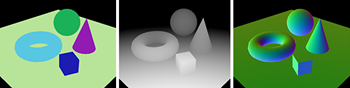
\includegraphics[width=4.85833in,height=1.21782in]{images/1_g_buffer.png}
		\caption{G-Buffer przedstawiający bufory koloru, głębi oraz wartości normalnych. \cite{tutsplus-deferred-2024}}
		\label{intro-deferred-shading}
	\end{figure}
	
	\item \textbf{Clustered shading}

	Znany także jako Forward+ lub Tiled Forward Rendering. Jest to nowa technika rysowania łącząca zalety Forward z optymalizacją pozwalającą na obsługę znacznie większej ilości świateł. Wykorzystuje do tego celu zależność, według której światła znajdujące się daleko od obiektów nie dostarczają wystarczającej ilości energii - a co za tym idzie światła -- aby poświęcać moc obliczeniową na ich wyliczanie. Pole widzenia dzielone jest na trójwymiarową siatkę klastrów o ustalonym rozmiarze. Następnie przechodząc w pętli po wszystkich światłach w scenie, określa które z nich mają wpływ na dany klaster, dodając je do listy świateł dla pola. Końcowym etapem jest rysowanie bardzo zbliżone do tradycyjnego Forward Rendering, lecz zamiast określania oświetlenia na podstawie wszystkich świateł w scenie określane jest ono jedynie na podstawie listy punktów światła, które mają wpływ na testowany punkt \cite{aortiz:clustered:2024}. Wizualizacja metody znajduje się na rys. \ref{intro-clustered-rendering}.

	Zaletą tej metody jest znaczne zmniejszenie ilości odczytów i zapisów do pamięci względem Deferred Shading z jednoczesnym zwiększeniem możliwości renderowania oświetlenia w porównaniu do klasycznego Forward Rendering. Nie rozwiązuje ona jednak problemu overdrawing'u, jedynie nieco go maskując. Do wydajnej pracy zalecana jest także obsługa Compute Shaders do wyliczania pokrycia klastrów przez oświetlenie, co wyklucza szybkie działanie na starszych platformach.

	\begin{figure}[htbp]
		\centering
		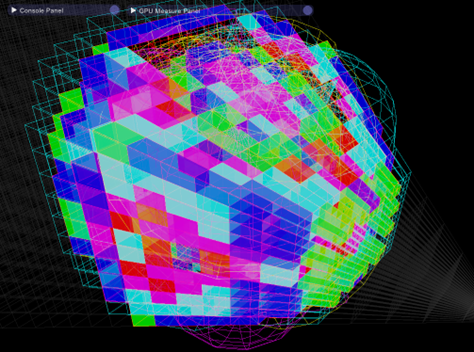
\includegraphics[width=4.94167in,height=3.67203in]{images/2_clustered_field.png}
		\caption{Podział pola widzenia na klastry. \cite{cnblogs:clustered:2024}}
		\label{intro-clustered-rendering}
	\end{figure}

	\item \textbf{Path Tracing}
	
	Technika śledzenia promieni (ang. Ray Tracing) jest najbardziej zbliżona do fizycznego modelu działania światła, co pozwala na uzyskanie bardzo realistycznych efektów. Z każdego punktu światła wysyłane są promienie światła, odbijając się od powierzchni obiektów, akumulując przy tym informacje o kolorze. Taki promień trafiając w sensor kamery przekazuje te informacje, które ostatecznie zostają zapisane na obraz docelowy. Taki model określa się mianem \emph{\textbf{Forward Path Tracing}}.
	
	Z perspektywy rysowania grafiki taka technika jest bardzo kosztowna obliczeniowo, gdyż zdecydowana większość promieni nie trafi do kamery, a zostanie rozproszona. W tym celu wykształciła się zoptymalizowana wersja techniki zwana \emph{\textbf{Backward Path Tracing}}. Różnica względem wariantu Forward polega na tym, że promienie śledzone są od kamery do światła, a nie odwrotnie. Jest to możliwe dzięki zasadzie wzajemności zaproponowanej przez Hermana Helmholtz'a, która głosi, że promień światła i jego odwrotność doświadcza takiej samej drogi oraz zjawisk fizycznych. \cite{wiki:helmholtz:2024}
	
	Technika ta pozwala na uzyskanie fotorealistycznych obrazów przy względnie prostym modelowaniu efektów, takich jak cienie, odbicia, refrakcję, głębię ostrości, okluzję otoczenia, czy symulowanie światła odbitego. Użycie Path Tracing'u w czasie rzeczywistym było bardzo rzadkie ze względu na jego koszt obliczeniowy. W 2018 roku firma NVIDIA wypuściła na rynek karty graficzne z serii RTX, które dodały funkcjonalność akceleracji sprzętowej obliczeń związanych z wykrywaniem kolizji promieni. Od tego czasu coraz więcej gier zaczęło korzystać z tej techniki celem poprawy jakości wyświetlanej grafiki.
\end{itemize}

\section{Modele cieniowania}

W celu realistycznego oddania świata rzeczywistego konieczne jest jak najdokładniejsze oddanie zachowania promienii świetlnych. Jednocześnie należy pamiętać o możliwej minimalizacji narzutu obliczeniowego celem poprawy wydajności.

\begin{itemize}
	\item \textbf{Cieniowanie płaskie}

	Najprostszy i najszybszy sposób cieniowania powierzchni. Oświetlenie wyliczane jest dla każdego wielokąta modelu, a następnie nakładane jako kolor danego poligonu.
	
	Wymaga bardzo małego nakładu obliczeniowego. Efekt jest wyraźnie nierealistyczny, sprawiając wrażenie ostrych krawędzi, co widoczne jest na rys. \ref{intro-flat-shading}. Mimo to bardzo dobrze oddaje on zależności między wielokątami, co jest przydatne na przykład w programach do modelowania grafiki 3D.

	\begin{figure}[htbp]
		\centering
		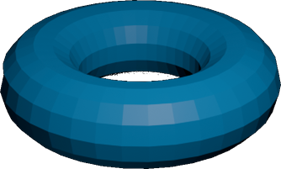
\includegraphics[width=3.90833in,height=2.34916in]{images/3_flat_shading_torus.png}
		\caption{Model torus'a narysowany przy pomocy cieniowania płaskiego.}
		\label{intro-flat-shading}
	\end{figure}

	\item \textbf{Cieniowanie Gouraud}
	
	Nazwana po autorze - Henri Gouraud -- technika cieniowania, w której natężenie światła wyliczane jest dla każdego wierzchołka, a następnie interpolowane dla fragmentów między tymi wierzchołkami. Charakteryzuje się niskim narzutem obliczeniowym i akceptowalnymi rezultatami. W przypadku modeli o niskiej rozdzielczości powoduje jednak powstawanie artefaktów, ze względu na kalkulacje oświetlenia jedynie dla wielokątów, których w takim przypadku jest niewiele, co widoczne jest na przykładowym obrazie widocznym na rys. \ref{intro-gouraud-shading}.

	\begin{figure}[htbp]
		\centering
		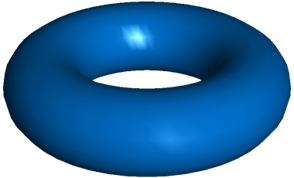
\includegraphics[width=4.08511in,height=2.475in]{images/4_gouraud_shading_torus.png}
		\caption{Model torus'a wygenerowany z użyciem cieniowania Gouraud i modelem światła Phong. \cite{wiki:gouraud:2024}}
		\label{intro-gouraud-shading}
	\end{figure}
	
	\item \textbf{Cieniowanie Phong}

	Model utworzony przez Bui Thong Phong na uniwersytecie Utah w 1973r. Poprawia niedokładność modelu Gouraud wykonując kalkulacje oświetlenia dla każdego fragmentu, a nie tylko wierzchołków. Efektem jest dobrze wyglądający model cieniowania pokazany na rys. \ref{intro-phong-shading}, z umiarkowanym kosztem obliczeniowym.
	
	Odbicia światła w tym modelu obliczane są na podstawie trzech parametrów widocznych na rys. \ref{intro-phong-components} - kolor otoczenia (ang. ambient), kolor rozproszony (ang. diffuse) używając modelu Lambertowskiego oraz tzw. specular reflection, obejmujący najjaśniejsze punkty odbite blisko lustrzanie.

	\begin{figure}[htbp]
		\centering
		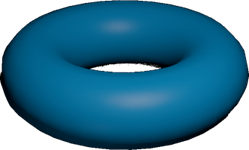
\includegraphics[width=3.45833in,height=2.08328in]{images/5_phong_shading_torus.png}
		\caption{Model torus'a wygenerowany z użyciem modelu cieniowania Phong.}
		\label{intro-phong-shading}
	\end{figure}
	
	\vfill
	\clearpage
	
	\begin{figure}[htbp]
		\centering
		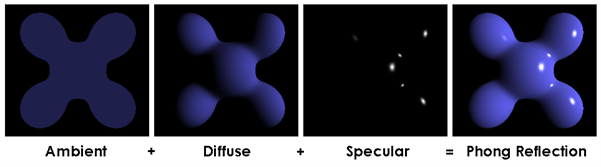
\includegraphics[width=6.25833in,height=1.74167in]{images/6_phong_shading_components.png}
		\caption{Komponenty składowe modelu Phong. \cite{wiki:phong:2024}}
		\label{intro-phong-components}
	\end{figure}
	
	\item \textbf{Model Blinn-Phong}
	
	Bazowy model Phong oblicza odbicia lustrzane (specular) poprzez wyznaczanie kąta między promieniem odbitym, a kamerą go obserwującą. Kąt ten jest następnie podstawiany do funkcji \emph{cos}, a wynik ograniczany do wartości z przedziału \textless0, 1\textgreater. Taki sposób kalkulacji ma jednak swoją wadę. W przypadku kątów większych od 90 stopni, wartość funkcji przyjmuje zawsze 0, co w przypadku bardzo chropowatych powierzchni może powodować artefakty, objawiające się jako twarde „odcięcie'' światła.
	
	Aby naprawić ten problem powstał model \emph{\textbf{Blinn-Phong}} zaproponowany przez James'a Blinn'a. Zamiast przeliczać bezpośrednio kąt odbicia do kąta kamery wyliczany jest wpierw kąt połowiczny między kątem padania światła i kątem obserwatora. Dzięki takiej modyfikacji oświetlenie zachowuje się bardziej naturalnie, bez znaczącego zwiększenia narzutu obliczeniowego.

	Model Blinn-Phong jest używany do obliczania odbić światła w starszych wersjach OpenGL i Direct3D używających \emph{Fixed Function Pipeline}.
	
	Różnice w obrazie wynikowym dla obu podejść można zobaczyć na rys. \ref{intro-phong-vs-blinn-phong}.
	
	\begin{figure}[htbp]
		\centering
		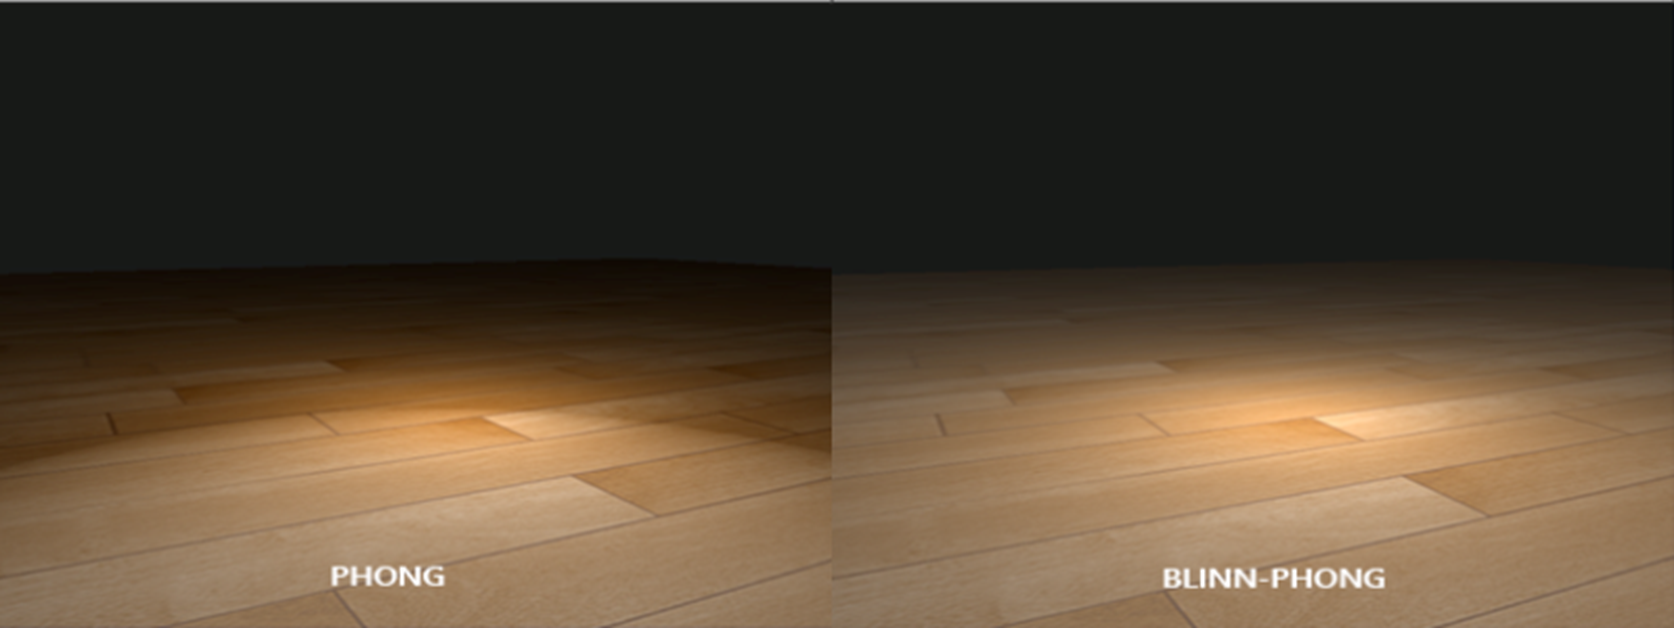
\includegraphics[width=5.58056in,height=2.09271in]{images/7_phong_vs_blinn_phong.png}
		\caption{Porównanie modelu Phong oraz Blinn-Phong dla bardzo chropowatej powierzchni i dużego kąta padania światła. \cite{learnopengl:advlighting:2024}}
		\label{intro-phong-vs-blinn-phong}
	\end{figure}
	
	\item \textbf{Physically Based Rendering}
	
	W skrócie \textbf{PBR}. Jest to grupa technik modelujących kalkulacje świetlne na podstawie prawdziwych zjawisk fizycznych. Ich niewątpliwą zaletą jest możliwość modelowania materiałów przy pomocy fizycznych właściwości obiektów bez uciekania się do sztuczek i aproksymacji.
	
	Systemy PBR najczęściej opierają się na modelu mikropowierzchni. Model taki aproksymuje zachowanie światła na mikroskopijnych nierównościach powierzchni obiektów. W przypadku równych materiałów światło będzie odbijało się w sposób bliski lustrzanemu, a chropowate powierzchnie będą je rozpraszać \cite{learnopengl:pbr:2024}, co widoczne jest na załączonym rys. \ref{intro-PBR}. Jest to zachowanie zbliżone do parametru chropowatości w opisanych wcześniej modelach.

	Drugim ważnym elementem systemu spełniającego założenie bazującego na rzeczywistości jest zasada zachowania energii. Ilość światła odbitego (a dokładniej jego energii) nie może przekraczać ilości włożonej energii. \cite{learnopengl:pbr:2024}

	Trzecim i ostatnim ważnym elementem opisywanego modelu jest funkcja typu BRDF (ang. Bidirectional Reflective Distribution Function). Przyjmuje ona jako parametry kierunek promienia światła \emph{\textbf{w\textsubscript{i}},} kierunek odbitego światła \emph{\textbf{w\textsubscript{o}}}, wektor normalny powierzchni \emph{\textbf{n}} oraz parametr \emph{\textbf{a}}, opisujący chropowatość powierzchni. Funkcja BRDF(w\textsubscript{i}, w\textsubscript{o}, n, a) aproksymuje ilość światła odbitego od powierzchni na podstawie jej parametrów \cite{learnopengl:pbr:2024}. Na przykład dla powierzchni lustra funkcja taka będzie zwracać 1 w przypadku kąta \emph{w\textsubscript{o}} będącego odbiciem \emph{w\textsubscript{o}}, a 0 w przeciwnym przypadku.
	
	\begin{figure}[htbp]
		\centering
		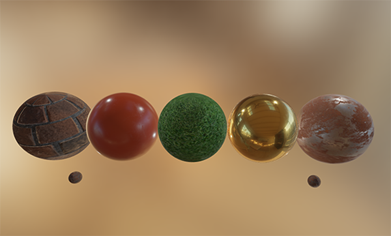
\includegraphics[width=5.425in,height=3.2752in]{images/8_pbr_surfaces.png}
		\caption{Powierzchnie cegły, plastiku, trawy, złota oraz zardzewiałego metalu wymodelowane przy pomocy PBR. \cite{learnopengl:pbr:2024}}
		\label{intro-PBR}
	\end{figure}
\end{itemize}

\section{Efekty graficzne poprawiające jakość obrazu}

Silniki renderujące oparte o klasyczne metody rysowania zmuszone są aproksymować zaawansowane efekty ze względu na ograniczenia tych metod. Poniżej opisane zostało kilka najpopularniejszych sposobów na poprawę jakości obrazu wynikowego.

\begin{itemize}
	\item \textbf{Wygładzanie krawędzi}

	Zjawisko \emph{\textbf{Aliasingu}} spowodowane jest ograniczeniami w metodach rasteryzacji obrazu przez karty graficzne. Wynika on z faktu, iż kolor pixeli na ekranie określany jest z odrębnych i nieciągłych punktów, czego efektem są ostre przejścia kolorów rysowanych obiektów i wrażenie „ząbkowania'' takich krawędzi.
	
	\item \textbf{MSAA}
	
	Najpopularniejszą metodą antialiasing jest \emph{\textbf{MSAA}} (ang. Multi-Sampling Anti Aliasing), czyli wielokrotne próbkowanie, której mechanizm działania został przedstawiony na rys. \ref{intro-msaa}. Jest to metoda akcelerowana sprzętowo przez współczesne karty graficzne, która jak nazwa wskazuje polega na wielokrotnym próbkowaniu z przesunięciem każdego pixela obrazu, a następnie wyciągania średniej jako ostatecznego koloru danego punktu. Technika ta wykazuje się dobrą jakością, ale jest względnie kosztowna obliczeniowo i nie jest możliwa w przypadku używania Deferred Shading.
	
	\begin{figure}[htbp]
		\centering
		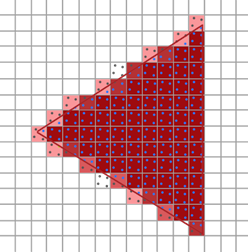
\includegraphics[width=3.4483in,height=3.5in]{images/9_MSAA_grid.png}
		\caption{Siatka reprezentująca działanie MSAA. Na niebiesko zaznaczone są punkty próbkowania, a czerwonymi liniami pokazane są krawędzie rysowanego obiektu. \cite{learnopengl:antialiasing:2024}}
		\label{intro-msaa}
	\end{figure}

	\item \textbf{TAA}
	
	\emph{\textbf{TAA}} (ang. Temporal Anti-Aliasing) jest uwspółcześnioną wersją MSAA. Zamiast wielokrotnego próbkowania pojedynczej klatki obrazu odbywa się ono na przestrzeni wielu, postępujących po sobie obrazach. Każdy proces rysowania rysuje obraz z lekkim przesunięciem punktów próbkowania pixeli, które następnie są uśredniane na potrzeby finałowego obrazu. Niewątpliwą zaletą tej techniki jest ograniczenie kosztu obliczeniowego, gdyż nie jest już wymagane wielokrotne próbkowanie pixeli. Pozwala ona także na użycie efektów \emph{dithering'u} do przezroczystości ze zmniejszoną ilością artefaktów. Z wad można wymienić narzut pamięci spowodowany koniecznością zapamiętywania poprzednich klatek, artefakty graficzne w postaci tzw. \emph{ghosting'u}, czyli pozostałości poprzednich klatek, a także widoczna nieostrość wynikowego obrazu.
	
	\item \textbf{FXAA}
	
	\emph{\textbf{FXAA}} (ang. Fast Aproximate Anti-Aliasing) operuje jako efekt post-procesowy w ścieżce generowania obrazu. Opracowany przez NVIDIA algorytm przetwarza obraz przez filtr górnoprzepustowy, wykrywając w ten sposób fragmenty obrazu o wysokim kontraście. Następnie metodami heurystycznymi znajduje w tych fragmentach krawędzie, które rozmywa przy pomocy kernel'a 3x3. Zaletą tej metody jest bardzo wysoka wydajność i brak narzutów pamięciowych. Jest to niestety też metoda dająca najsłabsze metody z wymienionych, powodując bardzo wyraźne rozmycie obrazu.
	
	\item \textbf{Odbicia środowiska}
	
	Aby dodać metalicznym i odbijającym światło obiektom głębi, należy dodać do silnika funkcjonalność obliczania odbić środowiskowych. Do najpopularniejszych metod należą:

	\item \textbf{Mapowanie sześcianów}

	Z angielskiego \emph{\textbf{Cube mapping}} jest techniką mapowania środowiskowego wykorzystującą do tego celu teksturę, zawierającą widok przestrzenny w 6 kierunkach, której przykładem jest rys. \ref{intro-cubemap}. Tekstura taka może być przygotowana z góry, z uwzględnieniem statycznych obiektów lub generowana w czasie rzeczywistym poprzez rysowanie geometrii z odpowiednich perspektyw. Tak przygotowany obraz nakładany jest następnie na rysowane obiekty w formie odbicia, co daje złudzenie realistycznego zjawiska.
	Taka metoda posiada jednak wiele wad. Generowanie sześciu obrazów co każdą klatkę prezentacji generuje bardzo wysokie koszty obliczeniowe. Można je zminimalizować zmniejszając jakość generowanego obrazu lub przeliczając jedynie kilka ścian na klatkę, ale zmniejsza to w efekcie jakość finalnego renderu. Przygotowane wcześniej cubemap'y omijają problemy z wydajnością, ale są z założenia statyczne, więc nie reprezentują zmian w otoczeniu. Dodatkowym ograniczeniem tej metody jest ograniczona dokładność odbić ze względu na różnice w generowanych mapach dla obiektów w różnych miejscach w przestrzeni. Sposobem obejścia tego problemu jest generowanie osobnych map dla różnych pomieszczeń bądź obiektów, ale wiąże się to z oczywistym narzutem obliczeniowym.
	
	\vfill
	\clearpage
	
	\begin{figure}[htbp]
		\centering
		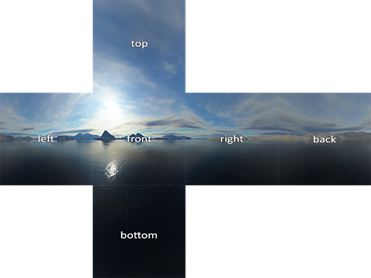
\includegraphics[width=5.14673in,height=3.85833in]{images/10_cubemap_environment.png}
		\caption{Przykład cubemap'y przedstawiającej tło środowiskowe.}
		\label{intro-cubemap}
	\end{figure}

	\item \textbf{Odbicia w przestrzeni ekranu}

	Z angielskiego \emph{\textbf{Screen-Space Reflection}} lub \emph{\textbf{SSR}}. Technika ta wychodzi z założenia, że większość odbić dotyczyć będzie obiektów, które zostały już wyrysowane, więc nie ma potrzeby renderowania ich po raz kolejny. W ten sposób ominąć można ograniczenia cubemap z jednoczesnym zachowaniem dostatecznej wydajności.

	Implementacja polega na wykonaniu pojedynczego śledzenia promienia w przestrzeni ekranu. Przyjmuje ona jako wejście bufory z teksturami kolorów, głębi oraz mapy odbijalności materiałów. Dla każdego fragmentu wykonuje pojedyncze śledzenie promienia na podstawie mapy głębi. Jeśli promień trafi na obiekt widoczny na ekranie, wykonywane jest jego odbicie, które następnie samplując po kolei z mapy głębi jest śledzone aż do trafienia obiektu. Jeśli tak się stanie, kolor trafionego materiału zostaje dodany jako odbicie do wyznaczanego koloru fragmentu. W przeciwnym wypadku za kolor odbity uznaje się światło nieba.
	Dużą zaletą tej techniki jest bardzo wysoka jakość odbić porównywalna do Ray-Tracing'u, szczególnie na płaskich powierzchniach pod dużym kątem, takich jak płaskie podłogi, czy powierzchnia wody. Z wad wymienić należy spory nakład obliczeniowy, a także artefakty, które powstają jeśli odbity promień trafi na obiekt nieznajdujący się w narysowanym obrazie.

	Przykład działania techniki został pokazany w ramach rys. \ref{intro-ssr}.

	\vfill
	\clearpage

	\begin{figure}[htbp]
		\centering
		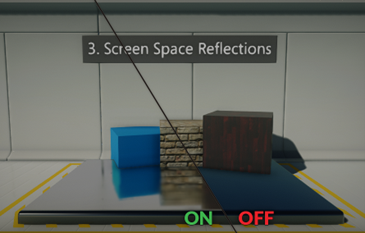
\includegraphics[width=5.06667in,height=3.2316in]{images/11_screen_space_reflections.png}
		\caption{Przykład działania Screen Space Reflections w porównaniu z brakiem tego efektu. \cite{flaxengine:ssr:2024}}
		\label{intro-ssr}
	\end{figure}

	\item \textbf{Ray Tracing}

	Najbardziej kosztowna wydajnościowo z opisywanych technik, ale dająca także najlepsze rezultaty, możliwe do zobaczenia na rys. \ref{intro-rt}. Opisana we wcześniejszym punkcie o Path Tracing'u metoda pozwala niskim kosztem dodatkowym uzyskać realistyczne odbicia bez ograniczeń \emph{SSR}. Podczas śledzenia promieni zliczany jest kumulowany kolor, co pozwala na uzyskanie odbić wielokrotnych, a także na rysowanie w odbiciach obiektów, które nie znajdują się na ekranie.

	\begin{figure}[htbp]
		\centering
		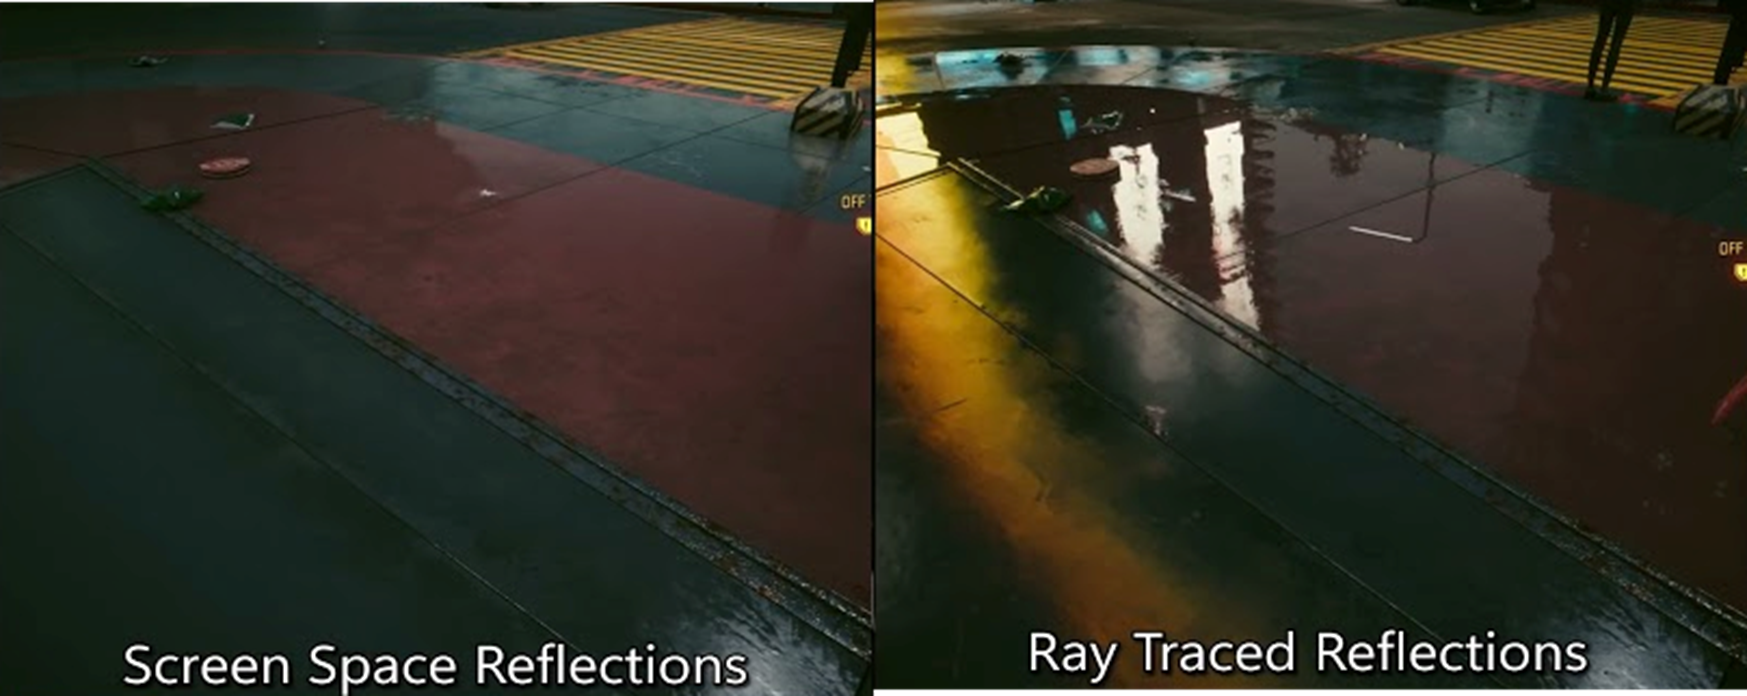
\includegraphics[width=5.82534in,height=2.32148in]{images/12_ssr_vs_rt.png}
		\caption{Porównanie Screen Space Reflections z odbiciami uzyskanymi techniką śledzenia promieni. \cite{niktek:reflections:2024}}
		\label{intro-rt}
	\end{figure}
	
	\vfill
	\clearpage
	
	\item \textbf{Ambient Occlusion}
	
	Okluzja otoczenia (ang. \emph{\textbf{Ambient Occlusion}}) jest techniką symulowania ograniczonej dostępności rozproszonego światła do kątów i zakamarków obiektów. Pozwala to na uzyskanie realistycznie wyglądającej aproksymacji prawdziwego zachowania światła.

	Do najpopularniejszych implementacji należą \emph{\textbf{SSAO}} (ang. Screen Space Ambient Occlusion), działający podobnie do \emph{SSR} oraz Path Tracing, który symuluje ten efekt symulując fizyczne zachowanie światła.
\end{itemize}

\section{Optymalizacja rysowania}

Poza dobrą jakością, bardzo istotnym elementem dobrego silnika renderującego jest także odpowiednia wydajność. Większość opisanych w poprzednim punkcie technik wyraźnie obciąża komputer rysujący, co zmusza do zastosowania technik optymalizacyjnych celem uzyskania dostatecznej szybkości działania. Poniżej opisane zostało kilka przykładowych, najczęściej stosowanych technik.

\begin{itemize}
	\item \textbf{Batching}

	Jednym z ograniczeń wydajności rysowania jest tzw. context switching, czyli zmiana używanego do rysowania shader'a i/lub materiału, a także ilość zapytań rysowania wysyłanych do karty graficznej. Aby zmniejszyć narzut wydajnościowy spowodowany takimi zmianami stosuje się technikę grupowania, czyli \emph{\textbf{Batching}}.
	Metoda ta dzieli się przede wszystkim na grupowanie statyczne i dynamiczne. Pierwsze wyliczane jest jeszcze przed uruchomieniem programu i dotyczy obiektów statycznych. Łączone są one w jeden, duży model i tak wysyłane w jednym zapytaniu do karty graficznej. Odmiana dynamiczna odbywa się przy rysowaniu w czasie rzeczywistym i sprowadza się do grupowania obiektów używających tego samego materiału do rysowania bezpośrednio po sobie, co pozwala uniknąć kosztownych zmian kontekstu. Metoda ta słabo nadaje się do obiektów używających różnych materiałów, gdyż wymagałoby to dostosowywania programów cieniujących do obsługi takiej techniki. Zupełnie brak jest możliwości łączenia ze sobą obiektów używających różnych shader'ów.

	\item \textbf{Frustum culling}

	Nie wszystkie obiekty sceny są widoczne w renderowanym jej fragmencie. Część znajduje się poza obszarem kamery, część jest zasłonięta przez wzgórza czy inne obiekty. W takim przypadku zbędną jest próba rysowania takich powierzchni, marnująć jedynie moc obliczeniową. Na pomoc wychodzi technika zwana \emph{\textbf{Frustum culling}}, pomijająca rysowanie niewidocznych obiektów na podstawie systemu wykrywania kontaktu ze stożkiem pola widzenia.
	Technika ta dzieli się na dwa zasadnicze podtypy. Pierwszym z nich, wykorzystywany klasycznie w silnikach idTech oraz Valve Source jest typ statyczny. W trakcie kompilacji mapy wyliczane są punkty widoczności na całej mapie, tak aby można było określić jakie fragmenty mogą być widoczne, a jakich nie trzeba rysować. Zaletą takiego rozwiązania jest bardzo wysoka wydajność, ale ograniczona jest ona do korytarzowej struktury pomieszczeń, gdyż na otwartych przestrzeniach ciężko mieć pewność co do widoczności w statycznej kalkulacji.
	Drugim sposobem jest typ dynamiczny. Przed rysowaniem klatki obrazu kalkulowane jest pokrywanie się obiektów sceny z fragmentem widocznym przez kamerę. Ze względu na wysoki koszt porównywania pełnych obiektów wykorzystuje się tzw. \emph{\textbf{Bounding Volumes}}, czyli figury geometryczne aproksymujące przestrzeń zajmowaną przez obiekt. Do najczęściej używanych należą sfery, prostopadłościany wyrównane do osi (AABB), czy prostopadłościany z rotacjami (OBB).
	W przypadku bardzo dużej ilości obiektów koszt obliczania elementów do narysowania wciąż może być zbyt duży. W tym celu wdrożyć można strukturę drzewową zwaną \emph{\textbf{Space partitioning}}, która dzieli rekursywnie przestrzeń na podfigury z informacją o ilości zawartych w nich obiektów. Następnie sprawdzając kolizje struktura taka umożliwia przejście „w dół'' drzewa, wykonując mniejszą ilość kalkulacji intersekcji. Najczęściej używa się drzewa z czterema podelementami dla gier 2D, ośmioma dla gier 3D, lub struktury \emph{\textbf{BSP}} (Binary Space Partitioning) jako optymalizacji dla większej ilości obiektów. System BSP używany jest we wspomnianych silnikach idTech oraz Valve Source.
	
	\item \textbf{Poziom detali}
	
	Z angielskiego \emph{\textbf{Level of Detail}} generuje dla każdego modelu jego alternatywne warianty ze zmniejszoną dokładnością i/lub ilością detali. W czasie rzeczywistym modele są podmieniane na niższej jakości wraz ze zwiększaniem się dystansu od kamery, co pozwala na uniknięcie rysowania nadmiernej ilości wielokątów w sytuacjach, w których użytkownik ma małą szansę ich zauważenia.
	
	\begin{figure}[htbp]
		\centering
		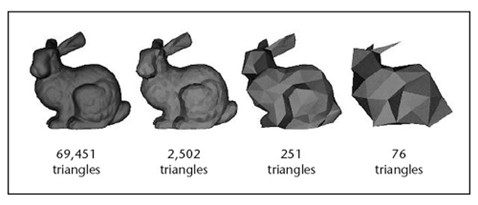
\includegraphics[width=4.975in,height=2.13971in]{images/13_LOD_rabbit.jpg}
		\caption{Poziom detali przedstawiony na modelu królika. \cite{3dstudio:lod:2024}}
	\end{figure}
\end{itemize}

\section{API graficzne}

Wydajny system renderujący powinien używać do rysowania akceleracji sprzętowej w postaci kart graficznych. W tym celu zalecanym jest użycie jednego ze wspieranych przez platformę API graficznych, które pozwalają na uzyskanie zamierzonego efektu bez konieczności dostosowywania kodu do konkretnych implementacji czy sprzętu. Wybór interfejsu powinien zależeć od zastosowania. Aplikacje celujące w starsze systemy będą miały odmienne wymagania do programów wyspecjalizowanych pod najszybsze komputery i najlepszą jakość grafiki. Nowsze API z reguły pozwalają na większą kontrolę nad procesem rysowania, ale kosztem złożoności ich użycia, a co za tym idzie czasem produkcji i skomplikowaniem korzystających z nich programów. Poniżej przedstawione zostało kilka przykładowych interfejsów.

\begin{itemize}
	\item \textbf{DirectX}

	Interfejs stworzony przez Microsoft dla platformy Windows i dokładniej opisany w następnym rozdziale. Jego najnowsza wersja -- DirectX 12 -- wspiera najnowsze rozszerzenia graficzne, takie jak DXR (DirectX RayTracing), VRS (Variable Rate Shading), Mesh Shaders czy DirectStorage.
	
	\item \textbf{OpenGL}

	Zaprojektowany w latach 90 przez Silicon Graphics stał się de facto standardem w dziedzinie interfejsów graficznych. Działa na zasadzie maszyny stanów, w której stan zapisywany jest po stronie sterownika graficznego. W pierwotnym wydaniu działający na zasadzie \emph{\textbf{Fixed Function Pipeline}}, a od wersji 3.1 opierający całe swoje działanie na modyfikowalnych ścieżkach rysowania. Najnowsza wersja to OpenGL 4.6. Wszystkie popularne systemy operacyjne wspierają ten standard z wyłączeniem Apple MacOS, który obsługuje jedynie do wersji OpenGL 4.1.

	\item \textbf{Vulkan}
	
	Sukcesor OpenGL zaprojektowany przez grupę Khronos. Względem swojego poprzednika rozszerza wsparcie o nowsze technologie, obsługę wielowątkowości oraz bardziej strukturalną konstrukcję. W dobrych rękach pozwala także na zmniejszenie narzutu obliczeniowego na procesor, a także zwiększenie wydajności renderowania poprzez możliwość określania przekazania sterownikowi bardziej dokładnych założeń co do modeli czy tekstur.
\end{itemize}

\section{Istniejące silniki graficzne}

Ze względu na duże zapotrzebowanie na rynku na różnego rodzaju programy do wyświetlania grafiki 2D i 3D, powstało wiele implementacji tego typu modułów. Część z nich można wykorzystać jako niezależne moduły renderujące, a część jest zintegrowana z konkretnym silnikiem graficznym bądź programem go wykorzystującym.

\begin{itemize}
	\item \textbf{Blender EEVEE}

	Stworzony na potrzeby programu do modelowania graficznego Blender silnik renderujący z założeniem działania w czasie rzeczywistym. Do rysowania grafiki korzysta z API OpenGL.

	Wspiera między innymi kalkulacje cieni metodami klasycznymi oraz przy pomocy Ray Tracing'u, oświetlenie wolumetryczne, oświetlenie globalne przy pomocy RT, a także efekty Post Process w postaci głębi ostrości, rozmycia w ruchu, czy Tonemapping'u z HDR do SDR.

	Przykład obiektu narysowanego przy pomocy EEVEE został pokazany na rys. \ref{intro-eevee}.

	\begin{figure}[htbp]
		\centering
		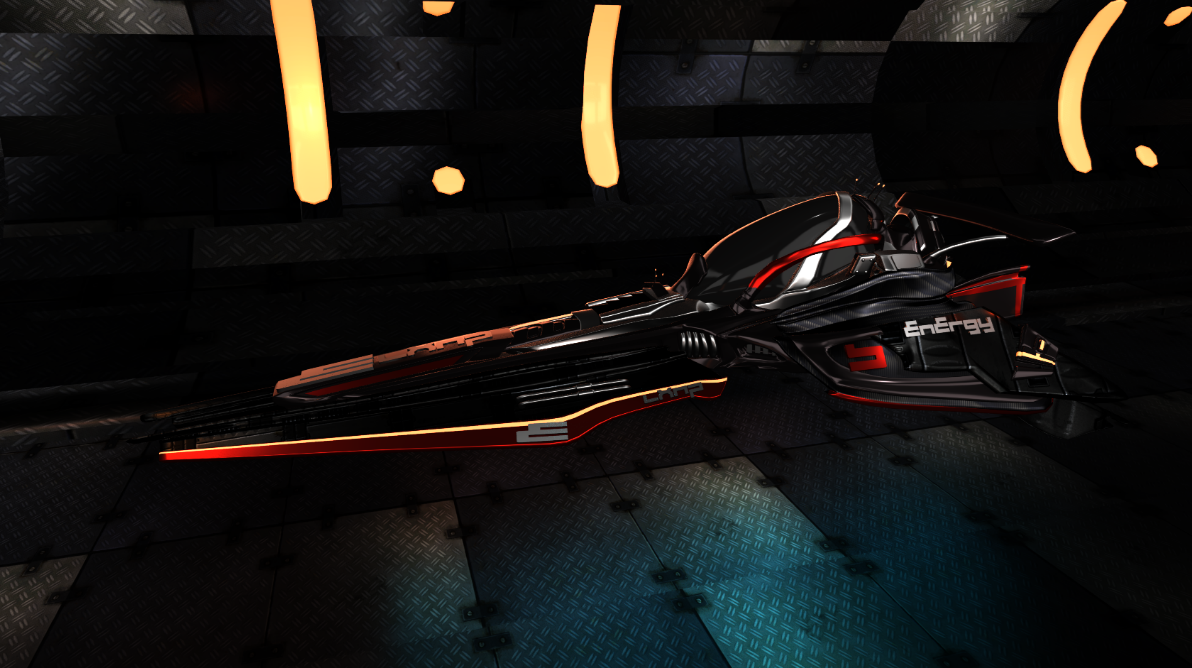
\includegraphics[width=5.41667in,height=3.03651in]{images/14_eevee.png}
		\caption{Obraz wygenerowany przy pomocy silnika EEVEE w programie Blender 4.2.1.}
		\label{intro-eevee}
	\end{figure}

	\item \textbf{Blender Cycles}

	Bardziej zaawansowany od EEVEE moduł stworzony z myślą o generowaniu fotorealistycznych renderów złożonej grafiki trójwymiarowej. Opiera swoje działanie na Path Tracing'u z wykorzystaniem akceleracji sprzętowej technologiami NVIDIA CUDA, NVIDIA OptiX, AMD HIP (RT), czy Intel oneAPI. Ze względu na charakterystykę algorytmu Path Tracing'u renderowanie z użyciem tego silnika wymaga bardzo dużej mocy obliczeniowej. W przeciwnym wypadku konieczne jest zmniejszenie ilości próbek dla każdego pixela, co powoduje ziarnistość obrazu wynikowego, widocznego na rys. \ref{intro-cycles-low}. Pomóc może dostępny w module system odszumiania obrazu.

	\vfill
	\clearpage

	\begin{figure}[htbp]
		\centering
		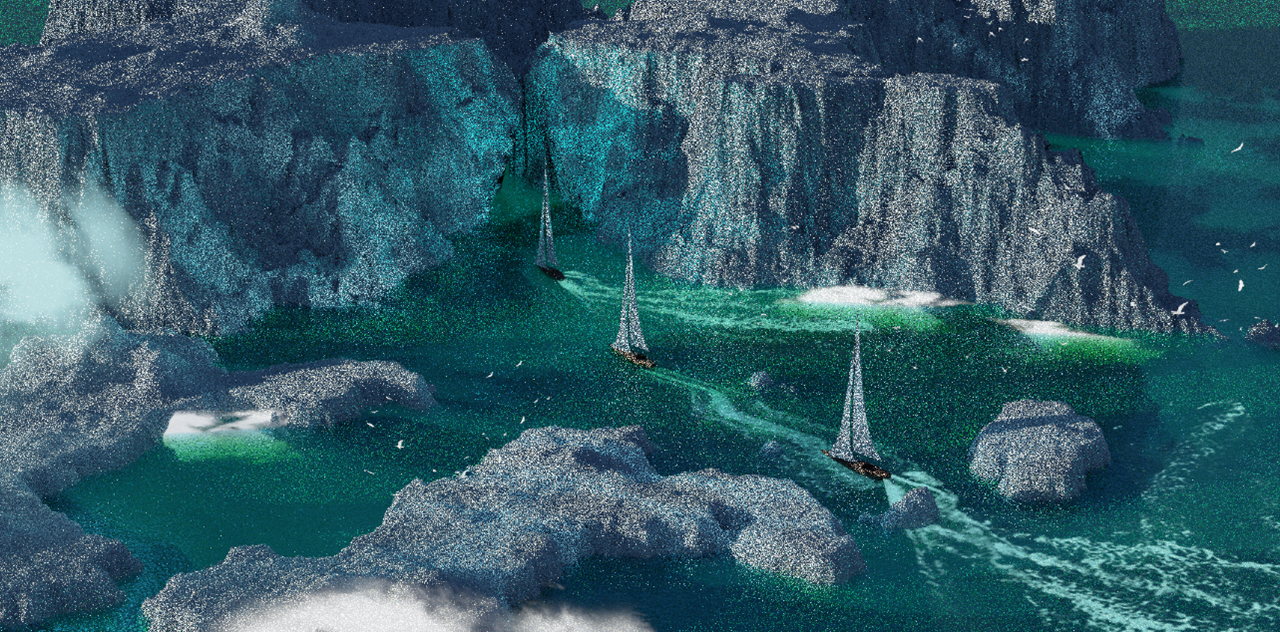
\includegraphics[width=5.81975in,height=2.875in]{images/15_cycles_low_samples.png}
		\caption{Obraz wygenerowany przez Cycles z niską ilością próbek, a przez to widocznym zaszumieniem.}
		\label{intro-cycles-low}
	\end{figure}

	Dzięki zastosowaniu metody śledzenia promieni do generowania obrazu, Cycles jest zdolny do generowania grafiki o bardzo wysokiej jakości i złożoności. Moduł ten poza funkcjami przejętymi od EEVEE posiada między innymi także pełną obsługę rozszerzonego standardu PBR, refrakcji i odbić światła, miękkich cieni, rozszerzonego globalnego oświetlenia w oparciu o system RT, przezroczystości, czy efektów wolumetrycznych także opartych o śledzenie promieni. Poprawnie wyrenderowany przy pomocy Cycles obraz został pokazany na rys. \ref{intro-cycles-high}.

	\begin{figure}[htbp]
		\centering
		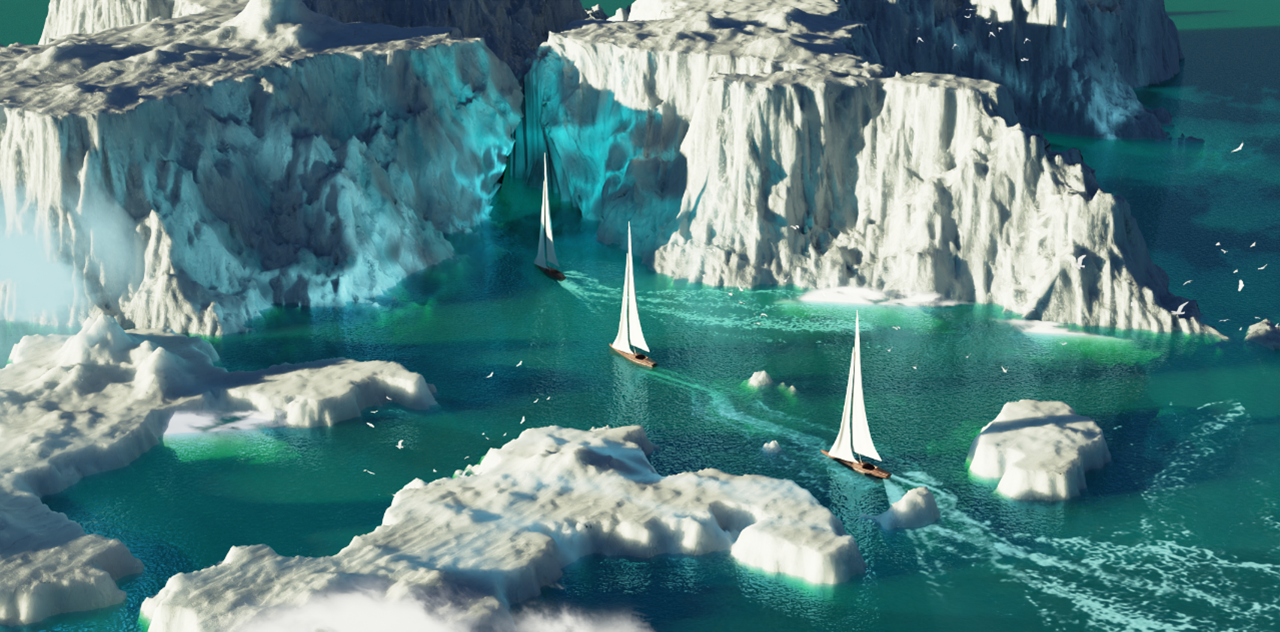
\includegraphics[width=5.81974in,height=2.875in]{images/16_high_samples.png}
		\caption{Obraz wygenerowany przez Cycles w programie Blender 4.2.1.}
		\label{intro-cycles-high}
	\end{figure}

	\vfill
	\clearpage

	\item \textbf{Unreal Engine}
	
	Silnik renderujący zastosowany w Unreal Engine jest jednym z najlepszych jakościowo dostępnych na rynku. Pozwala on na generowanie bliskich fotorealizmowi grafik w czasie rzeczywistym do zastosowania w grach. Oparty na systemie Deferred Shading posiada wiele zaawansowanych technik optymalizujących rysowanie obrazu. Najbardziej znanymi z nich są Lumen oraz Nanite. Pierwszy jest częściowo akcelerowanym sprzętowo algorytmem oświetlenia globalnego, pozwalającego na uzyskanie bardzo dobrych jak na standardy czasu rzeczywistego efektów względnie niskim kosztem obliczeniowym. Nanite natomiast zastępuje system Level of Detail, generując w czasie rzeczywistym fragmenty modeli o odpowiedniej jakości. Pozwala to na uzyskanie bardzo wysokiej szczegółowości modeli bez utraty wydajności związanej z systemem LOD. Oprócz opisanych technologii specyficznych, Unreal Engine obsługuje także między innymi akcelerowany sprzętowo Ray Tracing do obsługi odbić, cieni oraz Lumen, pełną obsługę PBR, czy subsurface scattering. Dzięki zastosowaniu RHI (Render Hardware Interface) czyli interfejsu abstrakcji, UE5 pozwala na skorzystanie z DirectX 11 oraz 12, OpenGL, jak i Vulkan do akceleracji graficznej. Nie wszystkie funkcjonalności są jednak dostępne w starszych API. 
	
	Przykład obrazu wygenerowanego przy pomocy Unreal Engine można zobaczyć na rys. \ref{intro-unreal-engine}.

	\begin{figure}[htbp]
		\centering
		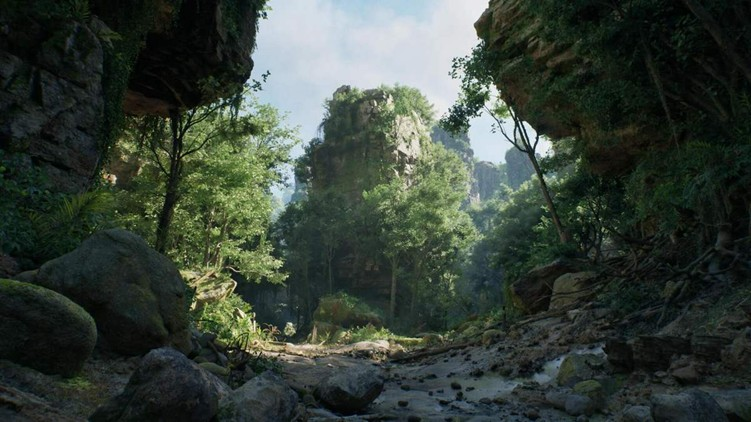
\includegraphics[width=5.21482in,height=2.93333in]{images/17_Unreal_engine_5_2.jpg}
		\caption{Klatka obrazu wygenerowana przez Unreal Engine 5.2.}
		\label{intro-unreal-engine}
	\end{figure}

	\item \textbf{Godot}

	W przeciwieństwie do większości popularnych silników graficznych, Godot nie korzysta z rysowania typu Deferred. Zamiast tego wykorzystywana jest technika Clustered Forward Rendering \cite{godot:rendererdesign:2024}. Technika ta została zastosowana ze względu na platformy docelowe opisywanego silnika, którymi są głównie mniej wydajne urządzenia mobilne, jak i uruchamianie aplikacji w przeglądarce przy użyciu WebGL.
	Architektura modułu także jest nieco odmienna od pozostałych. Jest on odrębnym podsystemem komunikującym się z głównym silnikiem jedynie poprzez pojedyncze gniazdo komunikacji. Przyjmuje jako argumenty parametry konfiguracyjne i strukturę opisującą scenę wraz z unikatowymi ID obiektów. Taka konstrukcja zmniejsza co prawda kontrolę programistów nad procesem rysowania, ale znacznie ułatwia rozwijanie kodu odpowiedzialnego za rysowanie. Ułatwia to także wsparcie dla różnych API graficznych.

	Silnik renderujący Godot posiada obsługę większości współczesnych efektów graficznych, takich jak Ambient Occlusion, Subsurface Scattering, Screen Space Reflections, czy efekty Post Process typu głębi ostrości, bądź rozmycia w ruchu. Moduł posiada także obsługę materiałów opartych o PBR. Nie celuje on jednak w wysoki fotorealizm, a bardziej w przystępną wydajność na słabszych urządzeniach. Przykładowym renderem za pomocą silnika Godot jest rys. \ref{intro-godot}.

	\begin{figure}[htbp]
		\centering
		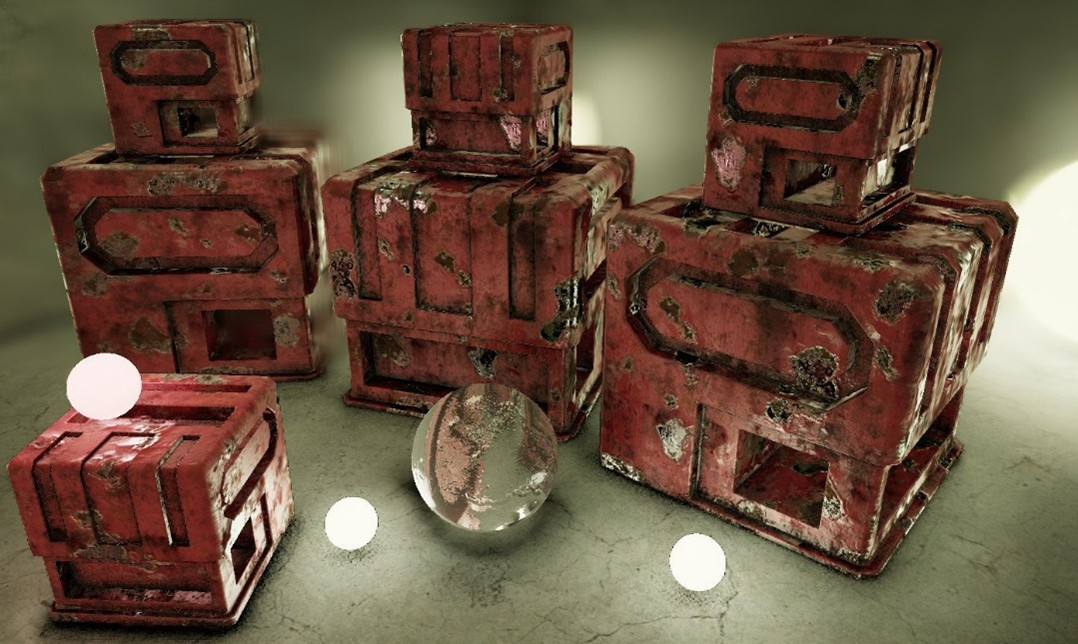
\includegraphics[width=4.90152in,height=2.92893in]{images/18_Godot_3_example.jpg}
		\caption{Klatka obrazu wygenerowana przez silnik Godot 3. \cite{godot:rendererdesign:2024}}
		\label{intro-godot}
	\end{figure}
\end{itemize}